%!TEX root = ../Thesis.tex
%% Basierend auf TeXnicCenter-Vorlage von Mark Müller
%%                      Willi Nüßer
%%                      Waldemar Penner     
%%                      Ulrich Reus
%%                      Frank Plass
%%                      Oliver Tribeß 
%%                      Daniel Hintze     
%%%%%%%%%%%%%%%%%%%%%%%%%%%%%%%%%%%%%%%%%%%%%%%%%%%%%%%%%%%%%%%%%%%%%%%

% Wählen Sie die Optionen aus, indem Sie % vor der Option entfernen  
% Dokumentation des KOMA-Script-Packets: scrguide

%%%%%%%%%%%%%%%%%%%%%%%%%%%%%%%%%%%%%%%%%%%%%%%%%%%%%%%%%%%%%%%%%%%%%%%
%% Optionen zum Layout des Artikels                                  %%
%%%%%%%%%%%%%%%%%%%%%%%%%%%%%%%%%%%%%%%%%%%%%%%%%%%%%%%%%%%%%%%%%%%%%%%
\documentclass[%
paper=A4,         % alle weiteren Papierformat einstellbar
fontsize=12pt,    % Schriftgröße (12pt, 11pt (Standard))
BCOR=12mm,         % Bindekorrektur, bspw. 1 cm
DIV=14,            % breiter Satzspiegel
parskip=half*,    % Absatzformatierung s. scrguide 3.1
headsepline,      % Trennline zum Seitenkopf  
%footsepline,     % Trennline zum Seitenfuß
%normalheadings,  % Überschriften etwas kleiner (smallheadings)
listof=totoc,     % Tabellen & Abbildungsverzeichnis ins Inhaltsverzeichnis      
%bibtotoc,        % Literaturverzeichnis im Inhalt 
%draft            % Überlangen Zeilen in Ausgabe gekennzeichnet
footinclude=false,% Fußzeile in die Satzspiegelberechnung einbeziehen 
headinclude=true, % Kopfzeile in die Satzspiegelberechnung einbeziehen 
final             % draft beschleunigt die Kompilierung
]
{scrartcl}

%\setuptoc{toc}{totoc} % Inhaltsverzeichnis ins Inhaltsverzeichnis

% Neue Deutsche Rechtschreibung und Deutsche Standardtexte
\usepackage[ngerman]{babel} 

% Umlaute können verwendet werden
\usepackage[utf8]{inputenc}   

% Echte Umlaute
\usepackage[T1]{fontenc} 

% Latin Modern Font, Type1-Schriftart für nicht-englische Texte
\usepackage{lmodern} 

% 1/2-zeiliger Zeilenabstand
\usepackage[onehalfspacing]{setspace}

% Für die Defenition eigener Kopf- und Fußzeilen
\usepackage{fancyhdr} 

% Für die Verwendung von Grafiken
\usepackage[pdftex]{graphicx}

% Bessere Tabellen
\usepackage{tabularx}

% Für die Befehle \toprule, \midrule und \bottomrule, z.B. in Tabellen 
\usepackage{booktabs}

% Erlaubt die Benutzung von Farben
\usepackage{color}

% Verbessertes URL-Handling mit \url{http://...}
\usepackage{url}

% Listen ohne Abstände \begin{compactlist}...\end{compactlist}
\usepackage{paralist} 

% Ausgabe der aktuellen Uhrzeit für die Draft-Versionen
\usepackage{datetime}

% Deutsche Anführungszeichen
\usepackage[babel,german=quotes]{csquotes}

% Konfiguration der Abbildungs- und Tabellenbezeichnungen
\usepackage[format=hang, font={footnotesize, sf}, labelfont=bf, justification=raggedright,singlelinecheck=false]{caption}

% Verbessert die Lesbarkeit durch Mikrotypografie
\usepackage[activate={true,nocompatibility},final,tracking=true,kerning=true,spacing=true,factor=1100,stretch=10,shrink=10]{microtype}  

% Zitate und Quellenverzeichnis
\usepackage[
    bibstyle=authoryear,
    citestyle=authoryear-fhdw,  
    giveninits=false,         % false = Vornamen werden ausgeschrieben
    natbib=true,
    urldate=long,             % "besucht am" - Datum
    %url=false,
    date=long,                
    dashed=false, 
    maxcitenames=3,           % max. Anzahl Autorennamen in Zitaten
    maxbibnames=99,           % max. Anzahl Autorennamen im Quellenverzeichnis
    %backend=bibtex           % Ggf. für ältere Distributionen bibtex verwenden
    backend=biber
]{biblatex}
  
% Bibliograpthy
\bibliography{library/c_vs_rust_vs_go}

% Keine Einrückung bei einem neuen Absatz 
\parindent 0pt 

% Ebenentiefe der Nummerierung
\setcounter{secnumdepth}{3}

% Gliederungstiefe im Inhaltsverzeichnis 
\setcounter{tocdepth}{3} 

% Tabellen- und Abbildungsverzeichnis mit Bezeichnung:
\usepackage[titles]{tocloft}

% Sourcecode-Listings
\usepackage{listings}

\usepackage{style/listings-rust} % Listing für Rust

% Bestimmte Warnungen unterdrücken
% siehe http://tex.stackexchange.com/questions/51867/koma-warning-about-toc
\usepackage{scrhack} 

%% http://tex.stackexchange.com/questions/126839/how-to-add-a-colon-after-listing-label
\makeatletter
\begingroup\let\newcounter\@gobble\let\setcounter\@gobbletwo
  \globaldefs\@ne \let\c@loldepth\@ne
  \newlistof{listings}{lol}{\lstlistlistingname}
\endgroup
\let\l@lstlisting\l@listings
\makeatother

\renewcommand*\cftfigpresnum{Abbildung~}
\renewcommand*\cfttabpresnum{Tabelle~}
\renewcommand*\cftlistingspresnum{Listing~}
\renewcommand{\cftfigaftersnum}{:}
\renewcommand{\cfttabaftersnum}{:}
\renewcommand{\cftlistingsaftersnum}{:}
\settowidth{\cftfignumwidth}{\cftfigpresnum 99~\cftfigaftersnum}
\settowidth{\cfttabnumwidth}{\cfttabpresnum 99~\cftfigaftersnum}
\settowidth{\cftlistingsnumwidth}{\cftlistingspresnum 99~\cftfigaftersnum}
\setlength{\cfttabindent}{1.5em}
\setlength{\cftfigindent}{1.5em}
\setlength{\cftlistingsindent}{1.5em}

\renewcommand\lstlistlistingname{Listingverzeichnis}
 
% Style für Kopf- und Fußzeilenfelder
\pagestyle{fancy}
\fancyhf{}
\fancyhead[R]{\leftmark}
\fancyfoot[R]{\thepage} 
\renewcommand{\sectionmark}[1]{\markboth{#1}{#1}} 
\fancypagestyle{plain}{}

% Macro für Quellenangaben unter Abbildungen und Tabellen
\newcommand{\source}[1]{{\vspace{-1mm}\\\footnotesize\textsf{\textbf{Quelle:}} \textsf{#1}\par}}

% Anpassungen der Formatierung an Eclipse-Aussehen 
% http://jevopi.blogspot.de/2010/03/nicely-formatted-listings-in-latex-with.html
%\definecolor{sh_comment}{rgb}{0.12, 0.38, 0.18 } %adjusted, in Eclipse: {0.25, 0.42, 0.30 } = #3F6A4D
%\definecolor{sh_keyword}{rgb}{0.37, 0.08, 0.25}  % #5F1441
%\definecolor{sh_string}{rgb}{0.06, 0.10, 0.98} % #101AF9
% Für Druckausgabe sollte alles schwarz sein
\definecolor{sh_comment}{rgb}{0.0, 0.0, 0.0 }
\definecolor{sh_keyword}{rgb}{0.0, 0.0, 0.0 }
\definecolor{sh_string}{rgb}{0.0, 0.0, 0.0 }

\lstset{ %
  language=Java,
  basicstyle=\small\ttfamily,
  fontadjust, 
  xrightmargin=1mm,
  xleftmargin=5mm,
  tabsize=2,
  columns=flexible,
  showstringspaces=false,
  rulesepcolor=\color{black},
  showspaces=false,showtabs=false,tabsize=2,
  stringstyle=\color{sh_string},
  keywordstyle=\color{sh_keyword}\bfseries,
  commentstyle=\color{sh_comment}\itshape,
  captionpos=t,
  lineskip=-0.3em
}

%\makeatletter
%\def\l@lstlisting#1#2{\@dottedtocline{1}{0em}{1.5em}{\lstlistingname\space{#1}}{#2}}
%\makeatother

% Anhangsverzeichnis
\usepackage[nohints]{minitoc} %Anhangsverzeichnis

\makeatletter
\newcounter{fktnr}\setcounter{fktnr}{0}
\newcounter{subfktnr}[fktnr]\setcounter{subfktnr}{0}

\renewcommand\thesubfktnr{\arabic{fktnr}.\arabic{subfktnr}}
\newcounter{anhangcounter}
\newcommand{\blatt}{\stepcounter{anhangcounter}}

\newcommand{\anhang}[1]{\setcounter{anhangcounter}{0}\refstepcounter{fktnr}
\addcontentsline{fk}{subsection}{Anhang~\thefktnr: \hspace*{1em}#1}
\subsection*{{Anhang~\thefktnr \hspace*{1em} #1 \hspace*{-1em}}}
}

\newcommand{\subanhang}[1]{\setcounter{anhangcounter}{0}\refstepcounter{subfktnr}
\addcontentsline{fk}{subsubsection}{Anhang~\thesubfktnr: \hspace*{1em}#1}
\subsubsection*{{Anhang~\thesubfktnr \hspace*{1em} #1 \hspace*{-1em}}}
}

\newcommand{\anhangsverzeichnis}{\mtcaddsection{\subsection*{Anhangsverzeichnis \@mkboth{FKT}{FKT}}}\@starttoc{fk}\newpage}

% Links im PDF
\usepackage[pdfpagemode={UseOutlines}, plainpages=false,breaklinks=true,pdfpagelabels]{hyperref}

 % Abkürzungsverzeichnis
\usepackage[automake,
			acronym,         % create list of acronyms
            nonumberlist,
            toc, 
            section,
            nopostdot,  % avoid dot after acronym
            hyperfirst=false,% don't hyperlink first use
            %sanitize=none    % switch off sanitization as description % Deprecated
            ]{glossaries}
            \newglossarystyle{mylist}{%
\setglossarystyle{long}% base this style on the list style
\renewcommand*{\glossaryentryfield}[5]{%
    \glsentryitem{##1}\textbf{##2} & ##3 \\}%
}

% Verbessert das Referenzieren von Kapiteln, Abbildungen etc.
\usepackage[german,capitalise]{cleveref}

\makeglossaries\makeglossaries 
%Acronyms
\newacronym{AES}{AES}{Advanced Encryption Standard}
\newacronym{AI}{AI}{Artificial Intelligence}
\newacronym{AOA}{AOA}{Angle of Arrival}
\newacronym{API}{API}{Application Programming Interface}
\newacronym{ATM}{ATM}{Automated Teller Machine}

%Glossary
\newglossaryentry{Glossar}
{
	name=Glossar,
	description={Ein Glossar ist eine alphabetisch geordnete Liste von Begriffen aus einem bestimmten Wissensgebiet mit den dazugehörigen Definitionen.}
}


%%%%%%%%%%%%%%%%%%%%%%%%%%%%%%%%%%%%%%%%%%%%%%%%%%%%%%%%%%%%%%%%%%%%%%%
%% Parameter - Hier auf die eigene Arbeit anpassen
%%%%%%%%%%%%%%%%%%%%%%%%%%%%%%%%%%%%%%%%%%%%%%%%%%%%%%%%%%%%%%%%%%%%%%%

\newcommand{\studiengang}{Angewandte Informatik} 
\newcommand{\dokumententyp}{Studienarbeit}
\newcommand{\abgabedatum}{\today} 
\newcommand{\ort}{Paderborn} 
\newcommand{\fhdwstandort}{Paderborn} % oder Bielefeld, Mettmann, ...
\newcommand{\dokumententitel}{Darstellung der Weiterenwicklung von Programmiersprachen von C zu Rust und GO}
\newcommand{\dokumentenautor}{Celina Berends, Jan Löwen, Lennard Reinecke, Haiying Wang-Schulz}
\newcommand{\dokumentenpruefer}{Herr Nüßer}

%%%%%%%%%%%%%%%%%%%%%%%%%%%%%%%%%%%%%%%%%%%%%%%%%%%%%%%%%%%%%%%%%%%%%%%

\hypersetup{
  colorlinks=false,
  pdfborder={0 0 0},
  pdftitle=\dokumententitel,
  pdfauthor=\dokumentenautor
} 

\begin{document}

% Römische Seitennummerierung
\pagenumbering{Roman}
 
%%%%%%%%%%%%%%%%%%%%%%%%%%%%%%%%%%%%%%%%%%%%%%%%%%%%%%%%%%%%%%%%%%%%%%%
%% Titelseite
%%%%%%%%%%%%%%%%%%%%%%%%%%%%%%%%%%%%%%%%%%%%%%%%%%%%%%%%%%%%%%%%%%%%%%%

%!TEX root = ../Thesis.tex

\begin{titlepage}

\begin{center}

\includegraphics[scale=0.8]{img/fhdw}

\vspace{7mm}

\Huge{\bfseries\dokumententyp}\\

\vspace{5mm}

\LARGE{\dokumententitel}\\

\vspace{15mm}

\large{Prüfer(in):\\

\dokumentenpruefer\\

\vspace{15mm}

Verfasser(in):\\

\dokumentenautor\\

\vspace{3mm}

\vspace{7mm}

\studiengang\\

}

\enlargethispage{2em}

\vspace{15mm}

\large{Eingereicht am:\\

\abgabedatum \\

}

\end{center}


\end{titlepage}



%%%%%%%%%%%%%%%%%%%%%%%%%%%%%%%%%%%%%%%%%%%%%%%%%%%%%%%%%%%%%%%%%%%%%%%
%% Draft-Einstellungen
%%
%% Für die finale Version auskommentieren!
%%%%%%%%%%%%%%%%%%%%%%%%%%%%%%%%%%%%%%%%%%%%%%%%%%%%%%%%%%%%%%%%%%%%%%%
% \fancyhead[L]{\color{red} Stand: \today~-~\currenttime}

%%%%%%%%%%%%%%%%%%%%%%%%%%%%%%%%%%%%%%%%%%%%%%%%%%%%%%%%%%%%%%%%%%%%%%%
%% Verzeichnisse
%%%%%%%%%%%%%%%%%%%%%%%%%%%%%%%%%%%%%%%%%%%%%%%%%%%%%%%%%%%%%%%%%%%%%%%


% Sperrvermerk
%!TEX root = ../Thesis.tex
\section*{Sperrvermerk}
\addcontentsline{toc}{section}{Sperrvermerk}
\fancyhead[R]{Sperrvermerk}

Diese Arbeit enthält vertrauliche Informationen über die Firma \koorperationsunternehmen. Die Weitergabe des Inhalts dieser Arbeit (auch in Auszügen) ist untersagt. Es dürfen keinerlei Kopien oder Abschriften - auch nicht in digitaler Form - angefertigt werden. Auch darf diese Arbeit nicht veröffentlicht werden und ist ausschließlich den Prüfern, Mitarbeitern der Verwaltung und Mitgliedern des Prüfungsausschusses sowie auf Nachfrage einer Evaluierungskommission zugänglich zu machen. Personen, die Einsicht in diese Arbeit erhalten, verpflichten sich, über die Inhalte dieser Arbeit und all ihren Anhängen keine Informationen, die die Firma \koorperationsunternehmen{} betreffen, gegenüber Dritten preiszugeben. Ausnahmen bedürfen der schriftlichen Genehmigung der Firma \koorperationsunternehmen{} und des Verfassers.


Die Arbeit oder Teile davon dürfen von der FHDW einer Plagiatsprüfung durch einen Plagiatsoftware-Anbieter unterzogen werden. Der Sperrvermerk ist somit im Fall einer Plagiatsprüfung nicht wirksam.
\newpage
\fancyhead[R]{\leftmark}

% Inhaltsverzeichnis
\tableofcontents\newpage

% Glossar
\renewcommand{\glossarypreamble}{\label{glossary}}
\printglossary[style=long, title=Glossar, toctitle=Glossar] \newpage

% Abkürzungsverzeichnis
\renewcommand{\glossarypreamble}{\label{acronyms}}
\printglossary[type=acronym, style=long, title=Abkürzungsverzeichnis, toctitle=Abkürzungsverzeichnis] \newpage

\setcounter{table}{0} % printglossary erzeugt eine Tabelle, die die Nummerierung der "echten" Tabellen durcheinander bringt.

%%%%%%%%%%%%%%%%%%%%%%%%%%%%%%%%%%%%%%%%%%%%%%%%%%%%%%%%%%%%%%%%%%%%%%%
% Verzeichnisse
%%%%%%%%%%%%%%%%%%%%%%%%%%%%%%%%%%%%%%%%%%%%%%%%%%%%%%%%%%%%%%%%%%%%%%%

% Abbildungsverzeichnis
% \fancyhead[R]{\listfigurename}
% \listoffigures\newpage

% Tabellenverzeichnis
% \fancyhead[R]{\listtablename}
% \listoftables\newpage

% Quelltextverzeichnis
\fancyhead[R]{\lstlistlistingname}
\lstlistoflistings\newpage

% Kapitelüberschriften für den Arbeitstext
\fancyhead[R]{\leftmark}

%%%%%%%%%%%%%%%%%%%%%%%%%%%%%%%%%%%%%%%%%%%%%%%%%%%%%%%%%%%%%%%%%%%%%%%
%% Inhalt
%%%%%%%%%%%%%%%%%%%%%%%%%%%%%%%%%%%%%%%%%%%%%%%%%%%%%%%%%%%%%%%%%%%%%%%

% Arabische Seitennummerierung
\pagenumbering{arabic} 

\section{Einleitung}
\label{sec:Einleitung}

\section{Speicherverwaltung}
\label{sec:Speicherverwaltung}
In modernen Computersystemen ist Speicher ein vom Prozessor direkt zugreifbarer Hochgeschwindigkeitsspeicher, 
meist in Form von DRAM, der Programme und deren Daten speichert\autocite{OperatingSystemConcepts}. 
Da physischer Speicher schnell, aber begrenzt und flüchtig ist, wurde mit wachsender Programmgrösse 
und Mehrtasking-Betriebssystemen virtueller Speicher eingeführt.

Virtueller Speicher trennt den vom Programm wahrgenommenen logischen Adressraum vom physischen Speicher 
und vermittelt jedem Prozess den Eindruck eines grossen, zusammenhängenden Adressraums\autocite{OperatingSystemConcepts}. 
Durch Techniken wie Paging, Segmentierung und Demand Paging können Speicherbedarf und Sicherheit verbessert 
sowie Prozesse isoliert werden\autocite{IntroductionandOverviewoftheMulticsSystem}.

Die Speicherverwaltung koordiniert physische und virtuelle Speicherressourcen, weist Speicher zu, schützt Prozesse, 
wandelt Adressen um und lagert selten genutzte Daten aus, um eine effiziente und sichere Programmausführung in 
Mehrprozessumgebungen zu gewährleisten\autocite{Operating}.
\subsection{Speicherverwaltung basierend auf Programmiersprachen}
\label{sec:Speicherverwaltung basierend auf Programmiersprachen}
Speicherverwaltung ist nicht nur ein interner Mechanismus des Betriebssystems, sondern auch mit 
Programmiersprachen verknüpft. Aus der Perspektive der Implementierung von Programmiersprachen lassen sich 
zwei grundlegende Ansätze unterscheiden: manuelle Speicherverwaltung und automatische Speicherverwaltung.

\subsubsection{Manuelle Speicherverwaltung}
\label{sec:Manuelle Speicherverwaltung}

Manual Memory Management bezeichnet ein Verwaltungsmodell, bei dem die Zuweisung und Freigabe von Speicher 
während der Programmausführung explizit durch den Programmierer gesteuert werden und nicht automatisch durch 
die Laufzeitumgebung oder das Betriebssystem erfolgen\autocite{TheCProgrammingLaunguage}. In diesem Modell bestimmt der 
Entwickler mithilfe spezieller Funktionen zur Speicherzuweisung und -freigabe direkt den Lebenszyklus von 
Speicherblöcke im Heap. Das bedeutet, dass die Beschaffung, Nutzung und Freigabe von Speicher vollständig 
von der Logik und den Entscheidungen des Programmierers abhängen; Compiler und Laufzeitumgebung führen 
keine automatische Bereinigung nicht mehr genutzter Objekte durch.

In C verwendet man wie malloc(), calloc(), realloc() und free(), und 
in C++ wie new und delete verwendet werden, um den Speicherlebenszyklus 
im Heap direkt zu steuern. Dieses Verfahren bietet ein hohes Mass an 
Flexibilität und Vorhersehbarkeit: Entwickler können exakt festlegen, 
wann Speicher zugewiesen und freigegeben wird, und durch benutzerdefinierte 
Allokatoren oder Speicherpools die Leistung weiter optimieren\autocite{SmashingtheStackforFunandProfit}.

Allerdings bringt manuelle Verwaltung erhebliche Komplexität und Risiken mit 
sich. Da eine automatisierte Speicherbereinigung fehlt, führt das Versäumnis, 
nicht mehr benötigten Speicher rechtzeitig freizugeben, zu Speicherlecks, die 
bei langfristiger Ausführung die Systemressourcen erschöpfen können. Das Zugreifen 
auf bereits freigegebenen Speicher verursacht hängende Zeiger, was zu 
Programmabstürzen oder gar Sicherheitslücken führen kann\autocite{Seacord}. 
Darüber hinaus kann ein fehlerhaftes doppeltes Freigeben von Speicher die 
Heap beschädigen, während Pufferüberläufe zusätzliche Sicherheitsrisiken darstellen.

Trotz dieser Gefahren bleibt die manuelle Speicherverwaltung in Szenarien, 
die höchste Anforderungen an Leistung und Ressourcenkontrolle stellen, unverzichtbar 
wie in Betriebssystemkernen, eingebetteten Systemen oder im Hochleistungsrechnen.
\subsubsection{Automatische Speicherverwaltung}
\label{sec:Automatische Speicherverwaltung}

Automatische Speicherverwaltung bedeutet, dass nicht mehr genutzte Speicherobjekte 
durch einen Garbage Collection Mechanismus automatisch freigegeben werden, sodass 
der Programmierer den Speicher nicht manuell freigeben muss.

Speicherverwaltungsstrategien spiegeln tiefgreifend die Unterschiede im Designhintergrund, der 
Entwicklungszeit und den Zielanwendungsszenarien wider.

\subsection{Typische Speicherverwaltungsfehler in C}
\label{sec:Typische Speicherverwaltungsfehler in C}

Die Programmiersprache C wurde 1972 von Dennis Ritchie in den Bell 
Laboratories entwickelt, um portablen und effizienten Systemcode für 
das Unix Betriebssystem zu schreiben. Daher bietet C als frühe systemnahe 
Programmiersprache direkte Zugriff auf den Speicher und ein hohes Mass an Flexibilität. 
Gleichzeitig bringt der vollständig manuelle Speicherverwaltungsmechanismus von C 
jedoch zahlreiche potenzielle Risiken mit sich\autocite{TheCProgrammingLaunguage}.

Im vollständig manuellen Speicherverwaltungsmodell liegen Anforderung, Nutzung und 
Freigabe von Speicher vollständig in der Verantwortung des Entwicklers, während die 
Sprache selbst nahezu keine Laufzeitprüfungen oder automatischen Schutzmechanismen 
bereitstellt. Dies führt dazu, dass C Programme besonders anfällig für 
Speicherverwaltungsfehler sind,insbesondere in komplexen Projekten oder mit 
mehreren Entwicklern arbeiten zusammen.

Im Folgenden werden einige typische Fehlerarten aufgeführt, die bis heute eine 
wesentliche Ursache für Probleme in Systemsoftware und Sicherheitslücken darstellen.

\subsubsection{Dangling Pointers}
\label{sec:Dangling Pointers}
Ein hängender Zeiger ist ein Zeiger, der auf bereits freigegebenen Speicher verweist. 
Da C keine Überprüfung der Gültigkeit von Zeigern durchführt, führt der weitere Zugriff 
auf diesen Speicherblock nach der Freigabe zu undefiniertem Verhalten, was sich in 
Datenkorruption oder Programmabstürzen äussern kann betonen bei der Implementierung eines Speichermanagers, dass die Weiterverwendung eines 
freigegebenen Zeigers zu den gefährlichsten Fehlern in der C gehört\autocite{TheCProgrammingLaunguage}.
\begin{figure}[htp]
    \centering
    \lstinputlisting[
        language=C,
        caption=Beispiel dangling pointer in C
    ]{img/dangling_pointer.c}
    \label{fig:dangling_pointer_in_c}
\end{figure}

\subsubsection{Double Free}
\label{sec:Double Free}
Wenn derselbe Zeiger mehrfach mit free() aufgerufen wird, kann dies die Heap
beschädigen und zu Laufzeitfehlern oder Sicherheitslücken führen. Solche Defekte 
sind insbesondere in Multithread-Umgebungen besonders gefährlich, da Angreifer 
durch sorgfältig gestaltete Eingaben double free ausnutzen können, 
um Heap Spraying durchzuführen oder beliebigen Code auszuführen.
\begin{figure}[htp]
    \centering
    \lstinputlisting[
        language=C,
        caption=Beispiel double free in C
    ]{img/tow_of_free.c}
    \label{fig:double_free_in_c}
\end{figure}

\subsubsection{Wild Pointers}
\label{sec:Wild Pointers}
Wenn ein Zeiger nach seiner Deklaration ohne Initialisierung verwendet wird, verweist 
er auf eine zufällige Adresse, was zu schwer vorhersehbarem Verhalten führen kann. 
Solche Fehler stellen ein ernstzunehmendes Sicherheitsrisiko dar.
\begin{figure}[htp]
    \centering
    \lstinputlisting[
        language=C,
        caption=Beispiel wild pointer in C
    ]{img/wild_pointer.c}
    \label{fig:wild_pointer_in_c}
\end{figure}

\subsubsection{Buffer Overflow}
\label{sec:Buffer Overflow}
Pufferüberläufe gehören zu den berüchtigtsten Sicherheitslücken in der Geschichte 
der Programmiersprache C. Da Standardbibliotheksfunktionen wie strcpy oder scanf 
die Grösse des Zielpuffers nicht überprüfen, kommt es leicht zu out of bounds Zugriffen. 
Angreifer können diese Schwachstelle ausnutzen, um den Stack zu manipulieren und den 
Programmsteuerfluss zu übernehmen\autocite{SmashingtheStackforFunandProfit}. \autocite{TheCProgrammingLaunguage}weisen 
bei der Beschreibung von String zwar prägnante Beispiele auf, verzichten jedoch auf 
Sicherheitsprüfungen der Grenzen – ein Umstand, der die unzureichende Berücksichtigung 
von Sicherheitsaspekten im frühen Design der C Library deutlich macht.
\begin{figure}[htp]
    \centering
    \lstinputlisting[
        language=C,
        caption=Beispiel wild pointer in C
    ]{img/wild_pointer.c}
    \label{fig:wild_pointer_in_c}
\end{figure}

\subsection{Rust}
\label{sec:Rust}
Gibt es eine Sprache, die so schnell ist wie C/C++, aber sicherer ist und 
viele typische Speicherfehler vermeidet?

Vor diesem Hintergrund wurde Rust im Jahr 2015 veröffentlicht mit dem Ziel, 
C/C++ als systemnahe Programmiersprache zu ersetzen und die Speichersicherheitsprobleme 
von C/C++ zu lösen, ohne dabei auf Leistung zu verzichten.

Rust verfolgt das Konzept der „Zero Cost Abstractions“\autocite{TheRustProgrammingLanguage}: Es behält eine Leistung bei, 
die mit C++ vergleichbar ist, bietet aber gleichzeitig fortschrittliche und sichere 
Programmierabstraktionen. 
Die Speicherverwaltung in Rust basiert auf drei Kernmechanismen: Ownership, Borrowing 
und Lifetimes. Jeder Wert kann zu einem bestimmten Zeitpunkt nur einen Besitzer haben, 
und sobald dieser Besitzer den Gültigkeitsbereich verlässt, wird der Wert automatisch 
freigegeben (Nach meinem Verständnis ist das ähnlich dem RAII-Prinzip in C++.). Wenn Datenzugriff erforderlich ist, 
geschieht dies über Leihen, wobei die Nutzung den Regeln der Lebensdauer unterliegt, damit die Daten 
während der Verwendung stets gültig bleiben. Der Compiler überprüft die Lebensdauern bereits zur 
Kompilierzeit und verhindert so hängende Zeiger oder ungültige Referenzen\autocite{TheRustProgrammingLanguage}. Darüber hinaus stellt Rust 
intelligente Zeiger wie Box, Vec, Rc, Arc bereit, die gängige Speicherverwaltungsmodelle 
kapseln und vereinfachen.

Im Gegensatz zu Go verwendet Rust Speicher automatisch durch sein Ownership-System,ohne Garbage Collection\autocite{TheRustProgrammingLanguage}, was die Leistung auf dem Niveau von C/C++ 
hält. Zudem bietet Rust ein starkes Typsystem, das viele Fehler bereits zur Kompilierzeit erkennt, 
und unterstützt funktionale Programmierparadigmen. Im Vergleich dazu kann C++ zwar ebenfalls durch 
Klassenkapselung „gefährlichen Code“ isolieren, erzwingt aber keine strikten Sicherheitsgrenzen Entwickler 
können jederzeit „über die Grenzen hinausgehen“. In Rust hingegen erzwingt der Compiler 
die Markierung von unsicherem Code und verlangt, dass externe APIs innerhalb des Typsystems sicher bleiben, 
was die Speicher und -Nebenlaufsicherheit erheblich verbessert.

So löst Rust das in C häufig auftretende Problem der \glqq{}dangling Pointer\grqq{}:

\begin{figure}[htp]
    \centering
    \lstinputlisting[
        language=Rust,
        caption=Beispiel dangling pointer in Rust
    ]{img/dangling_pointer.rs}
    \label{fig:dangling_pointer_in_Rust}
\end{figure}

In Folgendem Code weist \textbf{Box::new(1)}einen i32 auf dem Heap zu und gibt einen Smart 
Pointer vom Typ Box<i32> zurück. Beim Ausführen von return num wird das Eigentum 
von num an den Aufrufer p übertragen, wodurch die Entstehung eines Dangling Pointers 
vermieden wird. Sobald p den Gültigkeitsbereich verlässt, wird automatisch das 
Drop-Trait von Box aufgerufen, um den belegten Heap-Speicher freizugeben und so 
eine sichere automatische Ressourcenverwaltung zu gewährleisten.

\begin{figure}[htp]
    \centering
    \lstinputlisting[
        language=Rust,
        caption= Beispiel: Behebung dangling pointer-Fehler aus C in Rust
    ]{img/dangling_pointer.rs}
    \label{fig:dangling_pointer_in_Rust}
\end{figure}

\begin{figure}[htp]
    \centering
    \lstinputlisting[
        language=Rust,
        caption=Beispiel: Behebung double free-Fehler aus C in Rust
    ]{img/tow_of_free.rs}
    \label{fig:double_free_in_Rust}
\end{figure}

In dem obigen Code allokiert vec![0; 10] einen zusammenhängenden Speicherbereich 
im Heap, um 10 <i32> Elemente zu speichern, während auf dem Stack lediglich ein 
Zeiger auf diesen Heap-Speicher, die Länge und die Kapazität gespeichert werden. 
Wenn data den Gültigkeitsbereich verlässt, ruft der Vec automatisch seinen 
Destruktor auf, um den belegten Heap-Speicher freizugeben und dadurch eine sichere 
Speicherverwaltung zu gewährleisten.

\subsubsection{Golang}
\label{sec:Golang}
Aufgrund der Komplexität und langsamen Buildungszeiten der C++ Projekte bei 
Google wurde eine einfachere, effizientere und nebenläufigkeitsfreundliche Sprache 
benötigt. Golang wurde 2007 von Google veröffentlicht. Die Designziele sind: einfache 
und leicht erlernbare Syntax durch Weglassen komplexer C++ Eigenschaften wie Vererbung, 
Templates und Makros; schnelle Entwicklung durch schnelle Kompilierung, die eine Iteration 
ähnlich wie bei Skriptsprachen ermöglicht; Nebenläufigkeit im Fokus mit eingebauten Goroutines 
und Channels, die parallele Programmierung erleichtern; und speziell geeignet für den Einsatz 
auf Serversseite zum Aufbau großskaliger verteilter Systeme.


\begin{figure}[htp]
    \centering
    \lstinputlisting[
        language=go,
        caption= Beispiel: Behebung dangling pointer-Fehler aus C in Golang,
    ]{img/danling.go}
    \label{fig:dangling_pointer_in_Golang}
\end{figure}

Der obige Go-Code löst das in C häufig auftretende Problem mit Nullzeigern. 
Die Funktion dangling pointer gibt die Adresse der lokalen Variablen num zurück. 
Der Go-Compiler erkennt mithilfe der Escape-Analyse automatisch, dass die 
Adresse von num zurückgegeben wird, und verschiebt daher die Allokation 
von num vom Stack auf den Heap. Dadurch wird sichergestellt, dass der 
zurückgegebene Zeiger auf gültigen Speicher verweist. Im main Funktionsblock 
wird dieser Zeiger dereferenziert und ausgegeben, was korrekt den Wert 1 liefert 
und zeigt, dass der Zeiger sicher und gültig ist.
\begin{figure}[htp]
    \centering
    \lstinputlisting[
        language=go,
        caption= Beispiel: Behebung double free-Fehler aus C in Golang,
        inputencoding=latin1
    ]{img/tow_of_free.go}
    \label{fig:double_free_in_Golang}
\end{figure}

Go verwendet ein automatisches Garbage Collection System, das effektiv 
das in C durch manuelles Speichermanagement verursachte Problem des 
double free vermeidet, welches zu undefiniertem Verhalten oder sogar 
Programmabstürzen führen kann. Dadurch wird die Komplexität und das 
Risiko der Speicherverwaltung deutlich reduziert\autocite{TheGolangMemoryModel}. Im obigen Code wird 
der Speicher für das Slice mit make vom Go-Laufzeitsystem automatisch 
verwaltet. Indem die Variable auf nil gesetzt wird, wird die Referenz 
entfernt, sodass der Garbage Collector den nicht mehr genutzten Speicher 
zur geeigneten Zeit freigeben kann. Ein manuelles Aufrufen einer 
Freigabefunktion ist somit nicht erforderlich, wodurch das Risiko 
eines doppelten Freigebens vollständig ausgeschlossen wird.

Dieser Mechanismus nutzt die Escape Analyse des Go-Compilers und den nebenläufigen 
Garbage Collector zur Laufzeit. So wird sichergestellt, dass Variablen im richtigen 
Speicherbereich abgelegt und nach ihrer Lebenszeit sicher wieder freigegeben werden\autocite{TheGolangMemoryModel}. 
Dadurch macht die automatische Speicherverwaltung in Go die Entwicklung einfacher und sorgt ausserdem dafür, 
dass Programme stabiler und sicherer laufen - typische Speicherfehler, wie man sie aus anderen Sprachen kennt, 
werden so vermieden.



\section{Parallelität}
\label{sec:Parallelität}

Mit der Zunahme an Kernen in modernen Prozessoren macht die parallele Gestaltung 
von Quellencode immer relevanter. Jedoch birgt die parallele Programmierung
auch einige Herausforderungen für den Programmierer mit sich. Programmiersprachen
können bei diesen Herausforderungen unterstützen oder dem Programmierer die Arbeit
erschweren. In diesem Abschnitt wird herausgearbeitet, wie Rust und Go den
Programmierer besser bei seiner Arbeit unterstützen als C.

\subsection{Parallelität in C}
\label{subsec:Parallelität in C}

Es wird begonnen die grundlegende Gestalung von Parallelität in C zu erläutern.
Zu diesem Zweck wird ein minimales Beispielprogramm in C erstellt, welches im 
Anhang \ref{anhang:vollstaendiger_quelltext} zu finden ist. 

In \cref{fig:datentyp_in_c} wird gezeigt, wie in C Threads initialisiert werden
und ihre Referenzen in einem Array gespeichert werden. In C gibt es nicht die 
Möglichkeit einen Thread ohne eine Referenz zu verwenden. Des Weiteren ist zu 
bemerken, dass in C Daten nur typenlos übergeben werden können und auch Resultate
können nur typenlos erhalten werden. Dies bedeutet, dass der Programmierer
selbst dafür sorgen muss, dass die Daten in der richtigen Form vorliegen. 
\autocite{hawthorneLanguageComparisonParallel}

\begin{figure}[htp]
    \centering
    \lstinputlisting[
        language=C,
        linerange={18-28},
        caption=Beispiel für die Verwendung Kollektionen zur Speicherung von Threads in C,
        label=fig:datentyp_in_c
    ]{img/parallelitaet_in_c.c}
\end{figure}

In \cref{fig:mutex_in_c} zeigt, dass um Synchronisation zu ermöglichen, muss
ein Mutex verwendet werden, um einen Codeabschnitt zu schützen. Prinzipell sind 
auch andere Synchronisationsmechanismen möglich, jedoch müssen diese vom 
Programmierer manuell angewendet werden. 

\begin{figure}[htp]
    \centering
    \lstinputlisting[
        language=C,
        linerange={10-14},
        caption=Beispiel für die Verwendung von Mutex in C,
        label=fig:mutex_in_c
    ]{img/parallelitaet_in_c.c}
\end{figure}


\subsection{Erweiterung in Go}
\label{subsec:Erweiterung in Go}
Im Kontrast zu C bietet Go mehr Unterstützung für das Programmieren mit Threads.
So zeigt \cref{fig:goroutinen}, dass in Go das Schlagewort \texttt{go} verwendet 
wird, um eine Goroutine zu starten, welche Equivalent zu einem Thread ist.

\begin{figure}[htp]
    \centering
    \lstinputlisting[
        language=go,
        linerange={16-23},
        caption=Beispiel für die Verwendung von Goroutinen in Go,
        label=fig:goroutinen
    ]{img/parallelitaet_in_go.go}
\end{figure}

Zur Synchronisation und Kommunikation zwischen Goroutinen bietet Go
Kanäle an. In \cref{fig:go_kanaele} kann gesehen werden, wie Daten über einen 
Kanal gesendet werden können. Dadurch das Kanäle in Go einen Datentyp erhalten,
hat der Programmierer mehr Sicherheit und eine leichere Handhabung. Des Weiteren
kann man mit Kanälen flexibeler die Kommunikation zwischen Goroutinen gestalten.
Dadruch dass Kanäle eine Buffergröße haben können, kann sowohl ein Mutex 
nachgestellt werden, wenn eine Buffergröße von 1 verwendet wird, als auch eine 
beabsichtigte Toleranz eingebaut werden, wie weit eine oder mehrere Goroutinen 
vorarbeiten dürfen, bevor sie auf das Lesen auf der anderen Seite des Kanals 
warten. \autocite{hawthorneLanguageComparisonParallel}

\begin{figure}[htp]
    \centering
    \lstinputlisting[
        language=go,
        linerange={25-28, 8-14},
        caption=Beispiel für die Verwendung von Kanälen in Go,
        label=fig:go_kanaele,
    ]{img/parallelitaet_in_go.go}
\end{figure}

\subsection{Erweiterung in Rust}
\label{subsec:Erweiterung in Rust}

Rust ändert die Grundsätzliche Verwendung von Threads nicht, deswegen ist eine 
ähnlichkeit der Struktur in \cref{fig:datentyp_in_c} und \cref{fig:rust_threads}
zu erkennen. Jedoch bietet Rust eine bessere Typensicherheit, da die Referenzen
von Daten, welche den Threads übergeben werden, nicht nur typisiert sind, sondern
auch der Arc-Typ verwendet. Dieser Arc-Typ ist ein Thread-sicherer 
Referenzzähler, welcher es ermöglicht, dass mehrere Threads auf die gleichen Daten
zugreifen können, ohne dass der Programmierer sich um die Synchronisation kümmern
muss. Dies wird bewekstäligt, inder der Arc-Typ erwartet, dass im ein Datentyp 
übergeben wird, welcher den \texttt{Send}-Trait und \texttt{Sync} implementiert. 
Diese Traits garantieren, dass der Datentyp sicher zwischen Threads 
übertragen werden kann und dass er von mehreren Threads gleichzeitig gelesen aber
nicht beschrieben werden kann.
\autocite{pfosiComparisonConcurrencyRust,IntroductionRustExample}

\begin{figure}[htp]
    \centering
    \lstinputlisting[
        language=Rust,
        linerange={9-26},
        caption=Beispiel für die Verwendung von Threads in Rust,
        label=fig:rust_threads,
    ]{img/parallelitaet_in_rust.rs}
\end{figure}

Des Weiteren bietet Rust die Möglichkeit, Daten über Kanäle zu senden, ähnlich
wie in Go mit der besonderheit, dass Rust Kanäle unidirektional sind im Gegensatz
zu Gos bidirektionale Kanäle. \autocite{ChannelsRustExample}

Ändere den Text

\section{Build Tooling}
\label{sec:Build_Tooling}

Buildsysteme und Tooling spielen eine zentrale Rolle in der Softwareentwicklung. Sie regeln, 
wie ein Projekt übersetzt wird, welche Abhängigkeiten es hat und wie es ausgeführt werden kann. 

C und C++ schneiden in diesem Bereich oft schlechter ab. Es gibt keine einheitliche Lösung, 
sondern eine Vielzahl unterschiedlicher Tools und Ansätze. Rust und Go versuchen, 
diese Schwächen zu vermeiden, indem sie ein klar strukturiertes und integriertes Tooling mitbringen.

\subsection{Tooling und Buildsysteme}
\label{subsec:Tooling_und_Buildsysteme}

In C und C++ existieren viele Buildsysteme, zum Beispiel Make, CMake, Autotools oder Meson. 
Welches davon ein Projekt verwendet, ist verschieden. Teilweise müssen auch eigene 
Skripte geschrieben werden, um alles zum Laufen zu bringen. Gerade bei plattformübergreifender 
Entwicklung oder beim Einstieg in bestehende Projekte führt das oft zu Problemen \autocite{SurprisinglyComplexWorld}.

Rust bringt mit cargo ein zentrales Werkzeug mit, das alles rund um den Buildprozess abdeckt. 
Es erkennt die Projektstruktur automatisch, führt Builds durch, verwaltet Abhängigkeiten, 
testet Code und erstellt Dokumentation, alles mit wenigen Befehlen \autocite{HelloCargoRust}. 
Eine zusätzliche Build-Konfiguration ist in vielen Fällen nicht nötig. 
Die Projektinformationen stehen in einer Datei namens Cargo.toml, die von cargo gelesen wird.

Auch bei Go ist kein externes Buildsystem nötig. Die Toolchain ist vollständig in die Sprache 
eingebaut. Mit Befehlen wie \texttt{go build} oder \texttt{go run} lassen sich Programme direkt 
übersetzen und starten, ohne dass vorher etwas konfiguriert werden muss. 
Solange eine Datei go.mod vorhanden ist, erkennt das System automatisch die Struktur 
und kann alle nötigen Schritte ausführen \autocite{UsingGoModules}.

Während C und C++ viel Freiheit lassen, setzen Rust und Go bewusst auf klare Standards. 
Beide Sprachen wollen damit typische Fehlerquellen vermeiden und die Einstiegshürde senken.

\subsection{Zentrale Paketregistrierung}
\label{subsec:Zentrale_Paketregistrierung}

Ein zentrales Problem bei C und C++ ist das Fehlen einer offiziellen Paketregistrierung. 
Zwar gibt es Werkzeuge wie vcpkg oder Conan, die eigene Repositories mitbringen, 
aber keine davon ist standardisiert oder universell verbreitet \autocite{NotesPackageManagement}. 
In vielen Projekten werden Abhängigkeiten manuell eingebunden, etwa durch Einbinden von Quellcode 
oder statische Bibliotheken. Das macht die Verwaltung aufwendig, besonders bei größeren Projekten 
oder wenn mehrere Teams beteiligt sind \autocite{tangUnderstandingThirdpartyLibrary2022}.

Rust geht hier einen anderen Weg. Mit crates.io gibt es eine zentrale, offizielle Plattform 
für Community- und Systempakete. Sie ist direkt in cargo integriert und wird standardmäßig verwendet, 
wenn Abhängigkeiten in der Cargo.toml eingetragen werden \autocite{HelloCargoRust}. Das macht es einfach, 
Pakete zu finden, zu installieren und aktuell zu halten, ohne zusätzliche Werkzeuge oder manuelle Downloads.

Auch Go nutzt eine zentrale Quelle, allerdings über einen Proxy. 
Standardmäßig verwendet die Toolchain proxy.golang.org, der als Cache zwischen Entwickler*innen 
und dem tatsächlichen Git-Repository dient \autocite{GoModulesReference}. 
Dieser Proxy verbessert die Stabilität und Verfügbarkeit, verhindert Breaking Changes 
und ermöglicht reproduzierbare Builds auch dann, wenn ein Repository offline geht.

Beide Sprachen zeigen, wie wichtig eine zentrale Anlaufstelle für Abhängigkeiten ist. 
Nicht nur zur Vereinfachung der Nutzung, sondern auch für Sicherheit, Transparenz und Wartbarkeit. 
C und C++ bieten solche Strukturen nur über Drittanbieter, was Fehler wahrscheinlicher macht.

\subsection{Paketmanager}
\label{subsec:Paketmanager}

In C und C++ gibt es keine standardisierte Lösung für die Verwaltung von Abhängigkeiten. 
Stattdessen haben sich mehrere verschiedene Paketmanager entwickelt, darunter z.B. vcpkg und Conan. 
Beide funktionieren unterschiedlich und bringen jeweils eigene Formate, 
Repositories und Tools mit \autocite{NotesPackageManagement}. Da kein System dominiert, 
muss bei jedem Projekt neu entschieden werden, welches Tool eingesetzt wird. 
Diese Situation erschwert die Zusammenarbeit zwischen Projekten und macht Wiederverwendbarkeit 
unnötig kompliziert \autocite{tangUnderstandingThirdpartyLibrary2022}.

Rust bringt seinen Paketmanager direkt mit: cargo. Das Tool ist eng mit der Paketregistrierung crates.io 
verbunden und installiert automatisch alle im Projekt angegebenen Abhängigkeiten. 
Dabei legt cargo ein Verzeichnis (target/) an, in dem alle kompilierten Artefakte landen, sowie ein Cargo.lock, 
das die exakten Paketversionen festhält. Auch Updates, lokale Pfade und optionale Features lassen sich direkt in 
der Cargo.toml konfigurieren \autocite{HelloCargoRust}.

Go verwendet mit „Go Modules" ein ähnliches System. 
Abhängigkeiten werden über go.mod definiert, automatisch heruntergeladen und im Modul-Cache gespeichert. 
Zusätzlich legt Go eine Datei go.sum an, die Prüfsummen der Abhängigkeiten enthält und so absichert, 
dass dieselben Versionen wiederverwendet werden \autocite{ManagingDependenciesGo}.

Sowohl Rust als auch Go setzen also auf eine enge Integration von Paketmanager, Registry und Buildsystem. 
Im Vergleich zu C/C++ sind damit weniger manuelle Schritte nötig, und es entsteht eine konsistentere Projektumgebung.

\subsection{Projektstruktur}
\label{subsec:Projektstruktur}

In C und C++ gibt es keine festgelegte Projektstruktur. Der Aufbau eines Projekts hängt stark vom 
verwendeten Buildsystem ab. Manche Projekte nutzen ein src/-Verzeichnis, andere verteilen Header 
und Implementierungsdateien frei über mehrere Ordner. Auch die Position von Konfigurationsdateien (z. B. CMakeLists.txt) 
variiert stark. Diese Flexibilität erlaubt zwar viele Freiheiten, führt aber oft zu Problemen, wenn man z.B. 
in ein fremdes Projekt einsteigt \autocite{SurprisinglyComplexWorld}.

Rust setzt auf eine klar vorgegebene Struktur. Ein Standardprojekt besteht aus einem src/-Ordner, 
einer Datei Cargo.toml und optional weiteren Unterverzeichnissen für Tests, Dokumentation oder Benchmarks. 
cargo erkennt diese Struktur automatisch, sodass Entwickler*innen sich nicht um die Einbindung einzelner Dateien kümmern müssen. 
Auch bei größeren Projekten mit mehreren Crates lässt sich die Struktur mithilfe von Workspaces gut organisieren \autocite{HelloCargoRust}.

Go verlangt keine bestimmte Struktur, solange es eine Datei go.mod gibt. 
Meistens liegt der Code direkt im Projektverzeichnis oder in einem cmd/- oder internal/-Ordner, 
aber die Sprache schreibt nichts explizit vor. Der \texttt{go build}-Befehl erkennt automatisch alle zugehörigen Dateien 
und baut das Projekt ohne weitere Konfiguration \autocite{UsingGoModules}.

Während C/C++ viel Entscheidungsfreiheit lassen, setzen Rust und Go bewusst auf einfache oder standardisierte Strukturen. 
Das erleichtert den Einstieg, macht Projekte besser wartbar und reduziert den Bedarf an zusätzlicher Dokumentation.

\subsection{Reproduzierbarkeit von Builds}
\label{subsec:Reproduzierbarkeit_von_Builds}

Ein häufiger Kritikpunkt an C und C++ ist die geringe Reproduzierbarkeit von Builds. 
Schon kleine Unterschiede in Compiler-Versionen, Abhängigkeiten oder Systempfaden können dazu führen, 
dass ein Projekt auf einem anderen Rechner nicht mehr zuverlässig kompiliert oder sich anders verhält. 
Zwar kann man mit viel Aufwand stabile Umgebungen aufbauen, etwa über Docker oder manuelle Dependency-Pinning-Strategien, 
aber ein einheitlicher Mechanismus fehlt \autocite{SurprisinglyComplexWorld}.

Rust nutzt Cargo.lock, um Reproduzierbarkeit sicherzustellen. Diese Datei wird beim ersten Build automatisch erzeugt 
und enthält die genauen Versionen aller verwendeten Pakete inklusive ihrer transitive Abhängigkeiten. 
Beim erneuten Build wird genau diese Version verwendet, solange sich Cargo.toml nicht ändert. 
Dadurch bleibt das Verhalten konsistent, selbst über verschiedene Systeme hinweg \autocite{HelloCargoRust}.

Go löst das Problem mit der Datei go.sum. Diese enthält Prüfsummen aller geladenen Abhängigkeiten und 
schützt so vor nachträglichen Änderungen im Repository. Zusammen mit go.mod stellt sie sicher, 
dass alle Entwickler*innen mit den gleichen Paketversionen arbeiten und Builds identisch verlaufen \autocite{ManagingDependenciesGo,UnderstandingGoModules}.

Beide Sprachen setzen damit auf integrierte Lösungen, um stabile und reproduzierbare Buildprozesse zu ermöglichen. 
Bei C und C++ muss diese Sicherheit hingegen extern hergestellt werden, was Zeit kostet und zusätzliche Fehlerquellen schafft.

\subsection{Plattformunabhängigkeit}
\label{subsec:Plattformunabhaengigkeit}

Plattformübergreifende Entwicklung ist in C/C++ grundsätzlich möglich, aber oft aufwendig. 
Viele Buildsysteme erzeugen unterschiedliche Artefakte je nach Betriebssystem, Compiler oder Umgebung. 
Auch das Einbinden von externen Bibliotheken unterscheidet sich stark zwischen Windows, Linux und macOS, 
etwa durch unterschiedliche Pfade, Bibliotheksformate oder Paketquellen. 
Paketmanager wie vcpkg oder Conan können zwar helfen, aber sie müssen korrekt eingerichtet werden 
und sind nicht in jeder Umgebung gleich zuverlässig \autocite{NotesPackageManagement,tangUnderstandingThirdpartyLibrary2022}.

Rust versucht, diese Probleme mit einer plattformübergreifenden Toolchain zu vermeiden. 
Die offizielle Rust-Distribution enthält bereits alles, was für den Build benötigt wird, 
und ist für alle gängigen Betriebssysteme verfügbar. cargo funktioniert auf allen Plattformen gleich, 
und auch die verfügbaren Pakete auf crates.io sind größtenteils systemunabhängig, 
solange sie keine nativen Bibliotheken einbinden \autocite{HelloCargoRust}.

Go geht ähnlich vor. Die Sprache und die gesamte Toolchain werden direkt von Google für verschiedene Plattformen bereitgestellt. 
Die Module werden plattformneutral verwaltet, und die Tool-Befehle (\texttt{go build}, \texttt{go get} usw.) 
funktionieren auf jedem unterstützten System gleich. Auch die Verwendung von Cross-Compilation ist in Go sehr einfach 
und standardmäßig verfügbar, was in C/C++ häufig nur mit erheblichen Anpassungen funktioniert \autocite{GoModulesReference,UsingGoModules}.

Im Vergleich zeigen Rust und Go, wie moderne Toolchains die Plattformunabhängigkeit deutlich verbessern können. 
Nicht durch externe Tools, sondern durch einen integrierten und standardisierten Ansatz. 
In C/C++ hingegen bleibt das Ziel zwar erreichbar, aber der Weg dorthin ist oft mühsam und fehleranfällig.

\subsection{Einstiegshürde und Entwicklerfreundlichkeit}
\label{subsec:Einstiegshuerde_und_Entwicklerfreundlichkeit}

Der Einstieg in C oder C++ ist aus Tooling-Perspektive oft schwierig. Neue Projekte erfordern zunächst die Wahl eines passenden Buildsystems, 
das Einrichten von Konfigurationsdateien und die Einbindung von Abhängigkeiten. Gerade für Einsteiger*innen ist es schwer abzuschätzen, 
welche Werkzeuge zusammenpassen, wie plattformübergreifende Builds funktionieren sollen und wie sich externe Bibliotheken 
integrieren lassen \autocite{SurprisinglyComplexWorld,NotesPackageManagement}. Selbst erfahrene Entwickler*innen brauchen oft viel Zeit, 
um bestehende Projekte zu verstehen und lokal lauffähig zu machen \autocite{tangUnderstandingThirdpartyLibrary2022}.

Rust nimmt Einsteigenden diese Entscheidungen weitgehend ab. Mit \texttt{cargo new} lässt sich ein vollständiges Projekt erzeugen, 
inklusive Ordnerstruktur, Manifest-Datei (Cargo.toml) und einer ersten main.rs. Abhängigkeiten werden automatisch heruntergeladen und eingebunden.
Auch für fortgeschrittene Anwendungsfälle wie Workspaces oder native Libraries gibt es klare Anleitungen \autocite{HelloCargoRust}.

Go geht sogar noch weiter und verzichtet fast vollständig auf Konventionen, die über das Notwendige hinausgehen. 
Ein neues Go-Projekt benötigt nur eine Datei go.mod, und mit \texttt{go build} oder \texttt{go run} kann der Code sofort getestet werden. 
Die Toolchain installiert automatisch alle benötigten Abhängigkeiten. Selbst komplexere Dinge wie Modulverwaltung 
oder Cross-Compilation sind in der Standardtoolchain enthalten und dokumentiert \autocite{UsingGoModules,UnderstandingGoModules}.

Beide Sprachen setzen also auf ein Tooling, das Entwickler*innen möglichst wenig Konfiguration abverlangt und schnell zu Ergebnissen führt. 
Das senkt die Einstiegshürde deutlich, besonders im Vergleich zu den teils komplexen Setups von C und C++.

\subsection{Zusammenfassung}
\label{subsec:Build_Tooling_Zusammenfassung}

C und C++ bieten beim Build Tooling wenig Einheitlichkeit. Es gibt viele verschiedene Tools, keine klare Standardlösung 
und vieles muss manuell konfiguriert werden. Das macht den Einstieg schwer und sorgt oft für Probleme bei der Zusammenarbeit.

Rust und Go lösen das anders. Beide Sprachen bringen von Anfang an ein zentrales Tool mit, das Builds, 
Abhängigkeiten und Projektstruktur übernimmt. Rust ist dabei etwas strukturierter und mächtiger, 
während Go möglichst einfach bleiben will. In beiden Fällen sorgt das dafür, dass Projekte schneller starten können, 
weniger Fehler entstehen und Builds besser nachvollziehbar bleiben.


\section{Fehlerbehandlung}
\label{sec:Fehlerbehandlung}
\subsection{Was ist Fehlerbehandlung und warum braucht man sie überhaupt?}
Fehlerbehandlung bezeichnet Mechanismen, um Fehler zu erkennen, zu melden und zu behandeln. Sie sorgt dafür, dass Programme zuverlässig funktionieren. Es gibt drei Arten von Fehlern: Bei Logikfehlern verhält sich das Programm durch fehlerhafte Programmierung der Anforderungen falsch. Es handelt sich also um semantische Fehler, die auf Ebene der Programmiersprachen nicht erkannt werden können. Kompilierfehler sind hingegen syntaktische Fehler, die vom Compiler erkannt werden und verhindern, dass das Programm überhaupt ausgeführt wird, zum Beispiel durch falsche Typzuweisungen. Hier ist es auf Ebene der Programmiersprachen wichtig, dass die Meldungen an den Programmierer gut lesbar und hilfreich sind. Zudem muss festgelegt werden, was überhaupt Kompilierfehler auslöst. In Go sorgt eine deklarierte, aber ungenutzte Variable für einen Kompilierfehler, in anderen Sprachen aber nicht. Der Fehlertyp, der auf der Ebene der Programmiersprachen am kritischsten ist, ist der Laufzeitfehler, also eine unerwartete Situation, die erst zur Laufzeit erkannt werden kann, wie das Fehlen einer Datei. Hier braucht es nicht nur lesbare Fehlermeldungen, sondern auch Fehlerbehandlungsmechanismen, die das Programm vor Ausfällen und Sicherheitslücken schützen.

\subsection{Fehlerrückgabe und -erkennung}
In C gibt es keine Konstrukte, die bei der Fehlerbehandlung unterstützen. Aus Erfahrung und Konvention haben die Anwender jedoch einheitliche Konstrukte entwickelt, mit denen Fehler erkannt und zurückgegeben werden können. Es werden Fehlerwerte zurückgegeben. Der eigentliche Rückgabewert der Methode wird in einen weiteren Speicherbereich geschrieben, der über einen Pointer mitgegeben wird.

\begin{figure}[htp]
	\centering
	\lstinputlisting[
	language=C,
	caption=Beispiel für die Verwendung von Errorcodes in C
	]{img/errorcodes.c}
	\label{fig:errorcode_in_c}
\end{figure}

Die Verwendung von Output-Parametern macht den Code weniger lesbar, da die Funktion nicht mehr durch ihre Deklaration automatisch dokumentiert ist, sondern das Lesen weiterer Dokumentation notwendig ist, um sie korrekt anzuwenden. Weiterhin muss die Funktion oder der Aufrufer absichern, dass der Parameter überhaupt auf einen Speicherbereich zeigt und dass der Output-Parameter nicht auf einen Eingabeparameter zeigt. Die Verwendung von Funktionen höherer Ordnung wie \texttt{map()} oder \texttt{filter()} wird unmöglich gemacht.

C++ führt deswegen Exceptions ein: Fehler werden über \texttt{throw}-Blöcke zurückgegeben, die die Funktion unterbrechen und über \texttt{try-catch}-Blöcke erkannt werden. Die Exception wird solange nach oben propagiert und der Stack abgewickelt, bis sie von einem passenden \texttt{catch}-Block gefangen wird. Die Fehlererkennung integriert sich mit dem objektorientierten Design der Sprache: Ein \texttt{catch}-Block kann spezifisch für eine Fehlerklasse beziehungsweise deren Untertypen implementiert werden, während andere Exceptions in einem anderen \texttt{catch}-Block behandelt werden. Die Fehler können so an der Stelle behandelt werden, an der der Entwickler es vorsieht. Eigentlicher Code und Fehlerbehandlungscode sind somit separiert und im Erfolgspfad gibt es keine zusätzlichen Kosten. Jedoch sorgen Exceptions dafür, dass jede Funktion einen undokumentierten Kontrollfluss haben kann, der schnell übersehen werden kann. Das Verlassen des normalen Kontrollflusses macht es unmöglich, Echtzeitanwendungen zu entwickeln. Weiterhin sind Exceptions teuer zu verwalten. Deswegen sind sie in sicherheitskritischen oder Embedded-Anwendungen häufig verboten.

\begin{figure}[htp]
	\centering
	\lstinputlisting[
	language=C++,
	caption=Beispiel für die Verwendung von Exceptions in C++
	]{img/exceptions.cpp}
	\label{fig:exceptions}
\end{figure}

Da dies also auch keine zufriedenstellende Lösung darstellt, implementieren Go und Rust Fehler als Werte wie in C, vermeiden jedoch Output-Parameter. In Rust gibt es algebraische Datentypen in Form von Enums, also Typen, die aus mehreren Varianten bestehen, sodass ein Wert des Enums eine konkrete Ausprägung annimmt. Zur Fehlerrückgabe werden die abstrakten Typen \texttt{Result<T,E>} mit den Ausprägungen \texttt{Ok<T>} und \texttt{Err<E>} sowie \texttt{Option<T>} mit den Ausprägungen \texttt{Some<T>} und \texttt{None}, die beide den \texttt{Try}-Trait implementieren, genutzt. Zur Fehlerbehandlung wird Pattern Matching eingesetzt, das erschöpfend sein muss, wodurch eine explizite Fehlerbehandlung gefordert wird. Will man den Fehler nicht sofort behandeln, kann man im Fehlerfall mit dem \texttt{?}-Operator den Fehler nach oben weiterreichen. Monadische Operationen erlauben es, durch Funktionen wie \texttt{map()} (wendet Funktion auf Wert an, wenn \texttt{Some}, sonst \texttt{None}) oder \texttt{and\_then()} (wie \texttt{map}, aber Funktion gibt selbst \texttt{Option<U>} zurück), fehlerbehaftete Berechnungen zu verketten, ohne ständig Fallunterscheidungen zu machen oder eine wachsende Typverkettung (zum Beispiel \texttt{Option<Option<Option<T>>>}) zu haben. Auf \texttt{Try}-Objekten kann auch \texttt{unwrap()} aufgerufen werden. Dies führt zu einem nicht wiederherstellbaren Fehler, der für einen Programmabbruch sorgt, wenn der Typ nicht der erfolgreiche (\texttt{Some}/\texttt{Result}) ist. Allgemein können diese Fehler mit dem \texttt{panic!}-Makro erzeugt werden.

\begin{figure}[htp]
	\centering
	\lstinputlisting[
	language=Rust,
	caption=Beispiel für die Verwendung des Try-Traits
	]{img/try.rs}
	\label{fig:try-rust}
\end{figure}

In Go werden Tupel aus Ergebnis und Fehlerwert zurückgegeben, wodurch der Entwickler auch hier gefordert ist, die Fehler explizit zu behandeln. Es fehlt jedoch eine Konstruktion wie das \texttt{?} in Rust, wodurch das häufige Weitergeben des Fehlers an vielen Stellen im Code wiederholt werden muss, was als umständlich wahrgenommen wird. Für nicht wiederherstellbare Fehler gibt es auch hier die \texttt{panic}-Funktionalität.

\begin{figure}[htp]
	\centering
	\lstinputlisting[
	language=Go,
	caption=Beispiel für die Verwendung von Tupeln
	]{img/tuple.go}
	\label{fig:tuple}
\end{figure}

\subsection{Aufräumen}
Neben Speicherbereichen, deren Freigabe durch Stack-Unwinding oder durch den Garbage Collector von der Programmiersprache selbst geregelt werden kann, halten Programme oft auch andere Ressourcen, wie zum Beispiel Datenbankverbindungen zur Persistierung. Ein wichtiger Teil der Fehlerbehandlung ist es, dass auch wenn das Programm nicht korrekt ablaufen kann, diese wieder freigegeben werden. In C gibt es keine Konstrukte, die den Programmierer hierbei unterstützen. In Rust und C++ wird das Prinzip „Resource Acquisition Is Initialization“ verwendet, das auch für die Freigabe von Speicherbereichen zuständig ist. Im Konstruktor eines Objekts werden alle Ressourcen akquiriert und im Destruktor wieder freigegeben. Dieser kann vom Entwickler überschrieben werden, sodass hier auch andere Ressourcen wieder freigegeben werden. Wenn Objekte den Geltungsbereich verlassen, wird der Destruktor auf jeden Fall aufgerufen. In C++ muss man jedoch darauf achten, dass der Destruktor keine Exception wirft, da sonst das Programm abgebrochen wird.

\begin{figure}[htp]
	\centering
	\lstinputlisting[
	language=C++,
	caption=Beispiel für die Verwendung von Destruktoren
	]{img/filewriter.cpp}
	\label{fig:raii}
\end{figure}

In Go funktioniert das RAII-Prinzip aufgrund der nicht-deterministischen Speicherfreigabe nicht. Jedoch kann durch das \texttt{defer}-Konstrukt Code definiert werden, der auf jeden Fall am Ende der Funktion aufgerufen wird, auch wenn die Funktion vor ihrem normalen Ende verlassen wird. So wird Code-Duplikation sowie das Vergessen von Ressourcenfreigaben vermieden.

\begin{figure}[htp]
	\centering
	\lstinputlisting[
	language=Go,
	caption=Beispiel für die Verwendung von defer
	]{img/defer.go}
	\label{fig:defer}
\end{figure}

\subsection{Fehlerisolation}
Bisher wurden nur Fehler behandelt, die es zulassen, wieder in einen normalen Zustand zurückzukehren. Manchmal ist dies aber nicht gewollt und der bisherige Programmablauf wird gestoppt. Zum Beispiel in Client-Server-Anwendungen ist gewollt, dass dann zwar der einzelne Client-Aufruf abstürzt, aber nicht gleich der gesamte Server mit abstürzt. Konstrukte zum Programmabbruch in C++ (\texttt{std::terminate}) und C (\texttt{abort}) verfügen nicht über eine solche Funktionalität. In Go kann im \texttt{defer}-Block \texttt{recover()} aufgerufen werden, das \texttt{panic} abfängt und eine Rückkehr zum normalen Programmfluss ermöglicht.

\begin{figure}[htp]
	\centering
	\lstinputlisting[
	language=Rust,
	caption=Beispiel für die Verwendung von catch\_unwind()
	]{img/catch_unwind.rs}
	\label{fig:catch_unwind}
\end{figure}

\subsection{Lesbarkeit}
Für eine gute Wartbarkeit ist es wichtig, lesbare Fehlermeldungen sowie einen Stack Trace zu haben, damit man schnell weiß, warum das Programm einen Fehler wirft. Hier kann zwischen Kompilierfehlern und Laufzeitfehlern unterschieden werden. Kompilierfehler kann man in einem kleinen Beispielprogramm vergleichen, in dem eine konstante Variable überschrieben wird. Hier erkennt man, dass Rust besonders hilfreich ist und neben der Fehlerquelle auch direkt eine Lösung mitliefert. Bei einem verschachtelten Laufzeitfehler, der zum Programmabbruch führt, geben Rust und Go einen Stack-Trace mit, während das C/C++-Programm einfach nur abbricht (siehe Folie 18/19 der Präsentation).

Auch bieten die Programmiersprachen Konzepte zum Loggen von Fehlern, die nicht zum Programmabbruch führen. In C gibt es die globale Variable \texttt{errno}, die von Funktionen gesetzt werden kann. Durch die \texttt{strerror()}-Funktion wird dieser Fehlercode in einen menschenlesbaren Text umgewandelt. Allerdings ist \texttt{errno} nicht auf allen Systemen threadsafe, wodurch es durch einen anderen Thread überschrieben werden kann, bevor es fertig verarbeitet wird. Außerdem ist die Ausgabe betriebssystemabhängig. In C++ implementieren Exceptions die Methode \texttt{what()}, die einen String zurückgibt. Kontext kann manuell mitgegeben werden.

\begin{figure}[htp]
	\centering
	\lstinputlisting[
	language=C,
	caption=Beispiel für die Verwendung von strerror(errno)
	]{img/errno.c}
	\label{fig:errno}
\end{figure}

\begin{figure}[htp]
	\centering
	\lstinputlisting[
	language=C++,
	caption=Beispiel für die Verwendung von Fehlermeldungen in Exceptions
	]{img/file.cpp}
	\label{fig:error_c++}
\end{figure}

Auch in Go gibt es das \texttt{error}-Interface, aus dem der Entwickler eigene Fehlertypen bauen kann, die mit der \texttt{Error()}-Funktion eine menschenlesbare Nachricht zurückgeben. Das \texttt{Unwrap}-Interface ermöglicht Fehlerketten. In Rust bietet der \texttt{Error}-Trait zusätzlich die Funktion \texttt{source()}, um Fehler zu verketten. Rust und Go bieten also eine Lesbarkeit Out-of-the-Box, die in C/C++ manuell hergestellt werden muss.

\begin{figure}[htp]
	\centering
	\lstinputlisting[
	language=Go,
	caption=Beispiel für die Verwendung von Fehlermeldungen in Go
	]{img/file.go}
	\label{fig:error_go}
\end{figure}

\begin{figure}[htp]
	\centering
	\lstinputlisting[
	language=Rust,
	caption=Beispiel für die Verwendung von Fehlermeldungen in Rust
	]{img/file.rs}
	\label{fig:error_rust}
\end{figure}


\section{Fazit}
\label{sec:Fazit}

	
%%%%%%%%%%%%%%%%%%%%%%%%%%%%%%%%%%%%%%%%%%%%%%%%%%%%%%%%%%%%%%%%%%%%%%%

%!TEX root = ../Thesis.tex
\section*{Anhang}
\addcontentsline{toc}{section}{Anhang}
\fancyhead[R]{Anhang}

\anhangsverzeichnis

\anhang{Vollständiger Quelltext}
\label{anhang:vollstaendiger_quelltext}

\begin{figure}[htp]
    \centering
    \lstinputlisting[
        language=C,
        caption=Beispiel für die Verwendung von Threads in C
        ]{img/parallelitaet_in_c.c}
    \label{ang:parallelitaet_in_c}
\end{figure}

\begin{figure}[htp]
    \centering
    \lstinputlisting[
        language=Go,
        caption=Beispiel für die Verwendung Goroutinen in Go
        ]{img/parallelitaet_in_go.go}
    \label{ang:parallelitaet_in_go}
\end{figure}

\begin{figure}[htp]
    \centering
    \lstinputlisting[
        language=Rust,
        caption=Beispiel für die Verwendung von Threads in Rust
        ]{img/parallelitaet_in_rust.rs}
    \label{ang:parallelitaet_in_rust}
\end{figure}

%!TEX root = ../Thesis.tex
\section*{Quellenverzeichnis}
\addcontentsline{toc}{section}{Quellenverzeichnis}
\fancyhead[R]{Quellenverzeichnis}

\defbibheading{mono}{\subsection*{Monographien}}
\defbibheading{mag}{\subsection*{Aufsätze in Sammelbänden und Zeitschriften}}
\defbibheading{art}{\subsection*{Zeitungsartikel}}
\defbibheading{web}{\subsection*{Internetquellen}}
\defbibheading{leg}{\subsection*{Rechtsprechung}}
\defbibheading{comp}{\subsection*{Unternehmensunterlagen/Gesprächsnotizen}}

\setlength\bibitemsep{1.5\itemsep}
\setlength{\bibhang}{2em}

\renewcommand{\baselinestretch}{1.50}\normalsize

\begingroup
\sloppy

\printbibliography[heading=mono,keyword=mono]
\printbibliography[heading=mag,keyword=mag]
\printbibliography[heading=web,keyword=web]

% Bei Bedarf einkommentieren: (erzeugt sonst Warnungen)
% \printbibliography[heading=art,keyword=art]
% \printbibliography[heading=leg,keyword=leg]
% \printbibliography[heading=comp,keyword=comp]

\endgroup


%%%%%%%%%%%%%%%%%%%%%%%%%%%%%%%%%%%%%%%%%%%%%%%%%%%%%%%%%%%%%%%%%%%%%%%

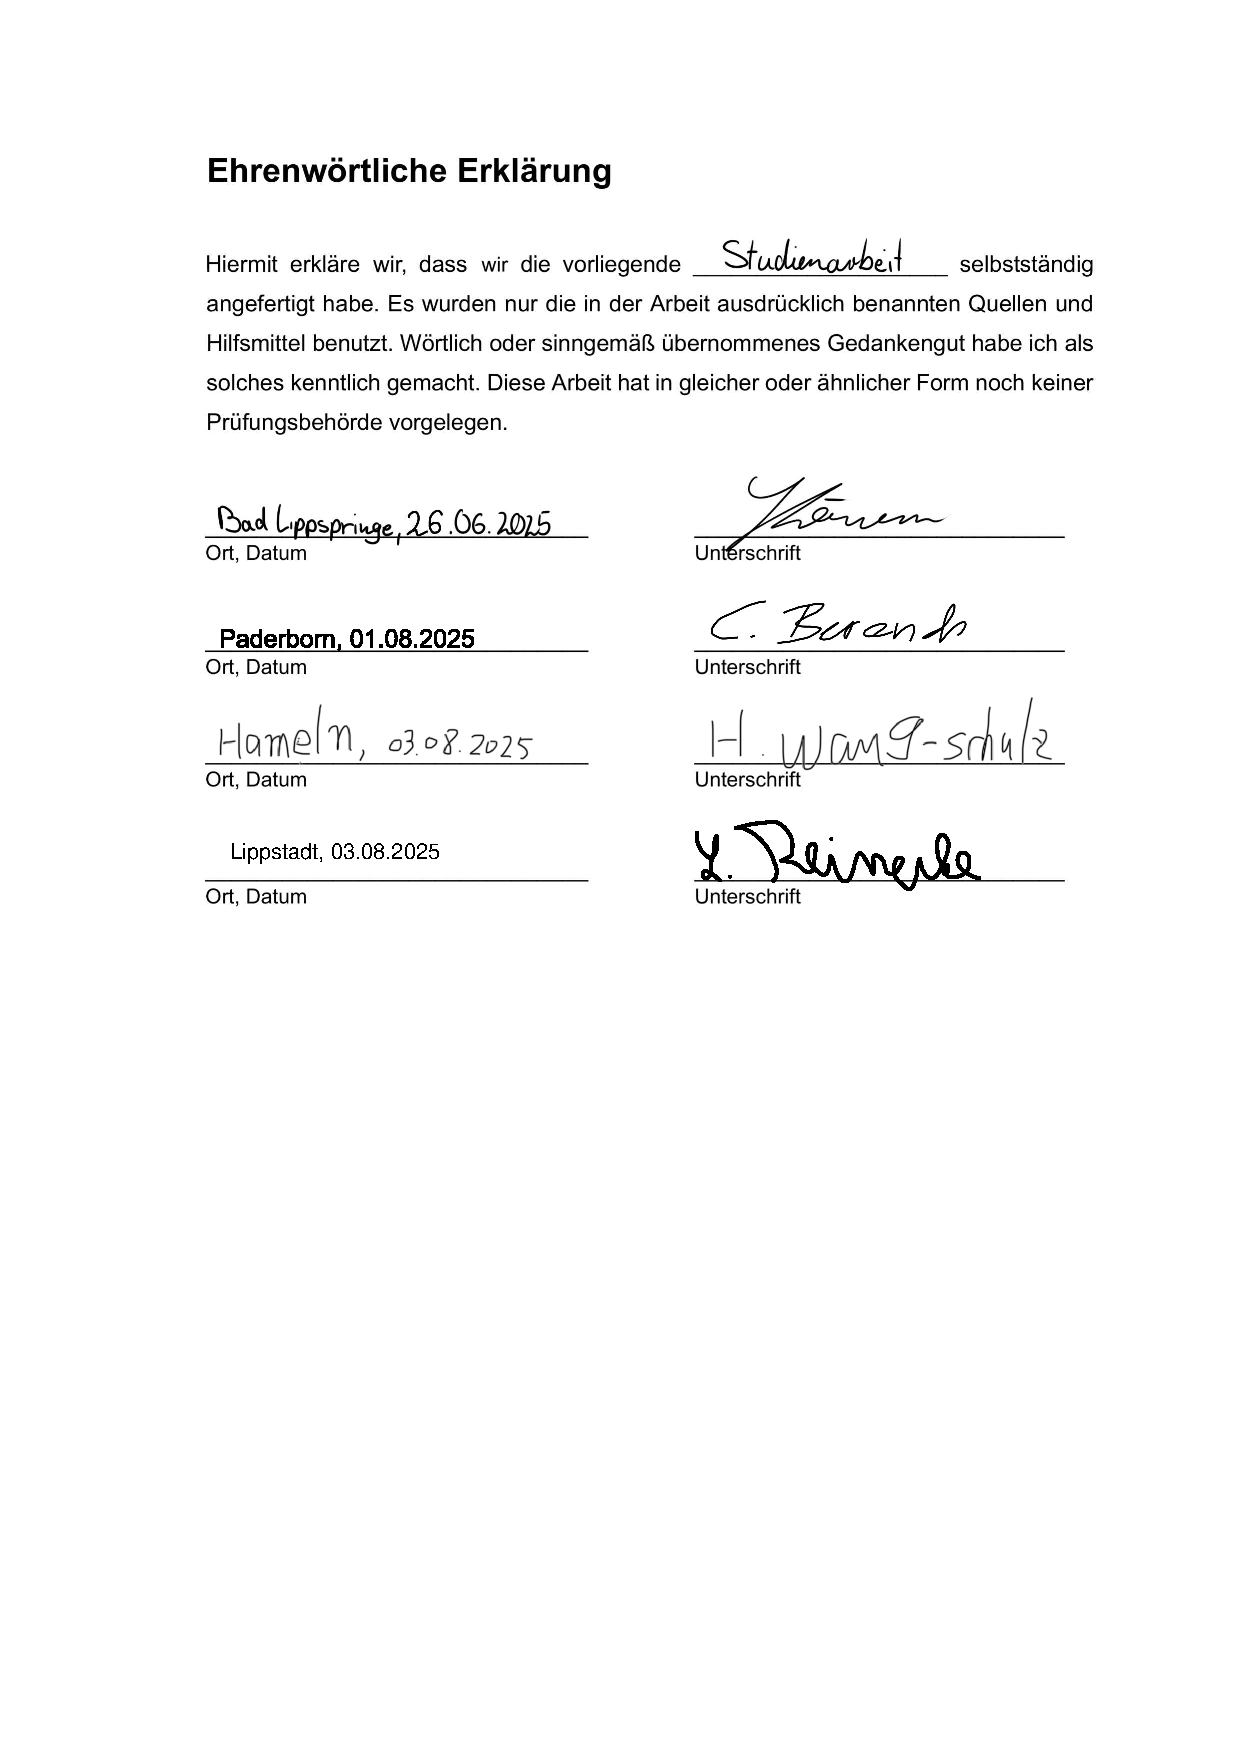
\includepdf{Ehrenwoertliche_Erklaerung}
 
%%%%%%%%%%%%%%%%%%%%%%%%%%%%%%%%%%%%%%%%%%%%%%%%%%%%%%%%%%%%%%%%%%%%%%%

\end{document}